\documentclass[twoside]{article}

\usepackage[hmarginratio=1:1,top=32mm,columnsep=20pt]{geometry} % Document margins
\usepackage[hang, small,labelfont=bf,up,textfont=it,up]{caption} % Custom captions under/above floats in tables or figures
\usepackage{booktabs} % Horizontal rules in tables

\usepackage{enumitem} % Customized lists
\setlist[itemize]{noitemsep} % Make itemize lists more compact
\usepackage{graphicx}
\usepackage{pdfpages}

\usepackage{xcolor}
\usepackage{fancyhdr} % Headers and footers
\pagestyle{fancy} % All pages have headers and footers
\fancyhead{} % Blank out the default header
\fancyfoot{} % Blank out the default footer
\fancyfoot[RO,LE]{\thepage} % Custom footer text
\font\myfont=cmr12 at 25pt
\font\myfon=cmr12 at 20pt

\usepackage{titling} % Customizing the title section

\usepackage{hyperref} % For hyperlinks in the PDF

%----------------------------------------------------------------------------------------
%	TITLE SECTION
%----------------------------------------------------------------------------------------

\setlength{\droptitle}{-4\baselineskip} % Move the title up

\pretitle{\begin{center}\Huge\bfseries} % Article title formatting
\posttitle{\end{center}} % Article title closing formatting
\title{\myfont CS310 Progress Report:\\ \myfon Efficient Allocation of Renewable Energy Sources Under Uncertainty Across the UK} % Article title
\author{James Page}


%----------------------------------------------------------------------------------------

\begin{document}

% Print the title
\maketitle

\section{Introduction}

In the first 8 weeks of this project, as planned, most of the progress made so far has been research to lay the groundwork for a smooth development stage. With this research done we can now refine our plans for the development. In this document we will highlight what new details we have to consider for the project and how what we have learnt has impacted the original plans for the project. Up to this point the schedule set out in the specification document (appendix of this document) has been followed without problem, so we will begin by examining the research done during this period. Following that we will use this information to determine what has changed with the plan and discuss why these changes are important to producing the best end product possible. Finally we will outline the next steps to be taken in the project and discuss our management approach to ensure we keep up a good pace.

%------------------------------------------------

\section{Research Progress}

When setting out on this project it was uncertain what types of renewable energy we would be examining after collecting a variety of sources we found that wind and solar generators had the most information available relevant to the UK, therefore the decision was made to start by focusing our research on these two areas.
%------------------------------------------------
\subsection{Energy Costs}
Information on the costs of installing solar photo-voltaic cells is extremely accessible as many people have looked to install small scale solar projects into their homes. However as we would be looking to install large scale solar farms with the scope of this project these price estimates may not scale accurately. To ensure we were making accurate estimations we ensured that any sources we used could be cross referenced with another accurate source. We found that the Renewable Power Generation Costs in 2019 report published by the International Renewable Energy Agency (IRENA) reported costs for everything we would need to know, reporting for Solar PV a cost of £1210 per kW on a commercial scale \cite{irena}. This would appear to be a very reliable source as it comes from a reputable agency trusted to keep track of many different aspects of renewable energy. Nevertheless we ensured that these numbers were consistent with a report published in 2019 by the UK government which estimated installations between 10-50kW (the upper end of their scale, so most relevant to a large scale commercial project) cost an average of £1139 per kW, and that this number had fallen to £1088 per kW by 2021.\cite{department_for_business_2021} This suggests to us that the IRENA report has accurate numbers to reference for costs overall even if prices will be slightly lower due to the year that has past since publication.
\\
\noindent The IRENA report also reports costs of installing onshore and offshore wind farms, with similar cost breakdowns of cost per kW to the solar reports. The reported cost of an offshore wind farm was reported as £3432 per kW in 2019 which is significantly more than installing solar panels. Onshore wind is not as expensive as offshore to set up but again is more expensive than a solar equivalent capcaity at £1349 per kW in Europe.\cite{irena}\\
However when you compare the levied cost of electricity from the generator, which is calculated by considering the operations and maintenance costs, lifetime capacity and the economic lifetime of the project (IRENA) we see that onshore wind is significantly cheaper than the other options at a cost of £0.0503 per kWh, compared to the £0.1403 per kWh and £0.0907 per kWh of solar photo-voltaics and offshore wind respectively \cite{irena}. This number does vary across different countries reported and solar may have a higher cost due it being relatively unused on a large scale in the UK and with increased adoption this may get better but currently this shows wind being the most efficient option to consider cost wise.
\subsection{Locations}
We found that generally with solar farms the location impact is fairly minimal over a small area like the UK, as the only impacting factor ends up being the levels of sunlight over a day. As such we decided that the due to location not being a huge factor in their performance we would narrow the scope to ignore solar power as it would only add complication to the end system without being a interesting problem to solve.
\\
\noindent When looking into suitable locations from wind farms another question comes up regarding the difference between offshore and onshore wind. In 2019 the UK had a slightly higher generation capacity of onshore wind than offshore, however the actual generation amounts were equal with both generating 9.9\% of the UK's total power each.\cite{energy_trends_mar2020} This is due to offshore farms having access to more suitable weather conditions resulting in a higher average load factor (average percentage of generation capacity actually generated) of 40.5\% compared to the 26.5\% of onshore wind\cite{energy_trends_mar2020}. From this it may appear advantageous to focus on offshore wind, and the increasing proportion of capacity being offshore over the last few years would also support this, but considering the levied cost of onshore wind farms being cheaper per kW generated \cite{irena} and that historical weather data is more readily available around onshore farms we will aim to focus on allocating onshore farms initially with this project with offshore being an area for expansion later.
\begin{figure}[!h]
    \centering
    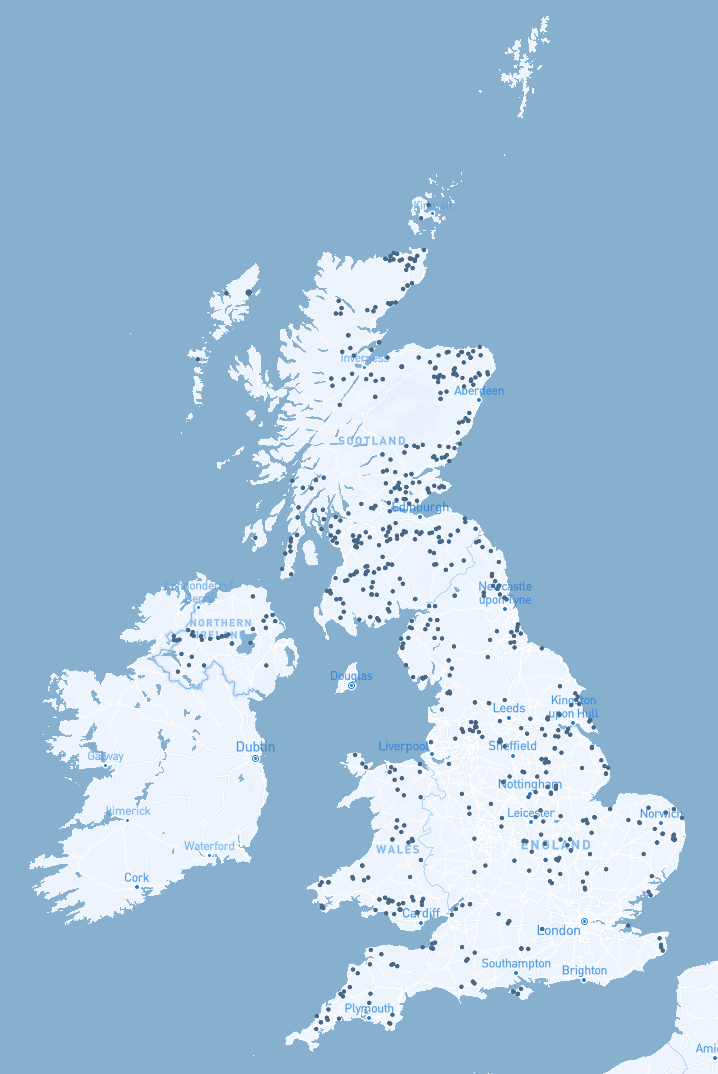
\includegraphics[height=200px]{RejectedWindApplications.png}
    \caption{Rejected Wind Farms UK 1990 - 2021, \cite{renew_database}}
    \label{fig:rejected_wind_farms}
\end{figure}
\\

\noindent Choosing a potential site to build a new wind farm is a difficult task as not just the generation can be considered, a perfect site may not be usable if you are not allowed to build there. Many wind projects get rejected as seen in \ref{fig:rejected_wind_farms} which shows all wind farm applications that have been refused recorded in the Renewable Energy Planning Database \cite{renew_database}. As such when deciding on locations we have decided to accept some limitations by only considering existing locations and suggesting the project finds the best of these existing projects to expand upon. This is a limitation that can be easily amended in future work if a list of suitable new sites is created. We will also be making use of locations that have been approved but are under or awaiting construction which expands our potential sites vastly as shown in \ref{fig:wind_farms}.

\begin{figure}[!h]
    \centering
    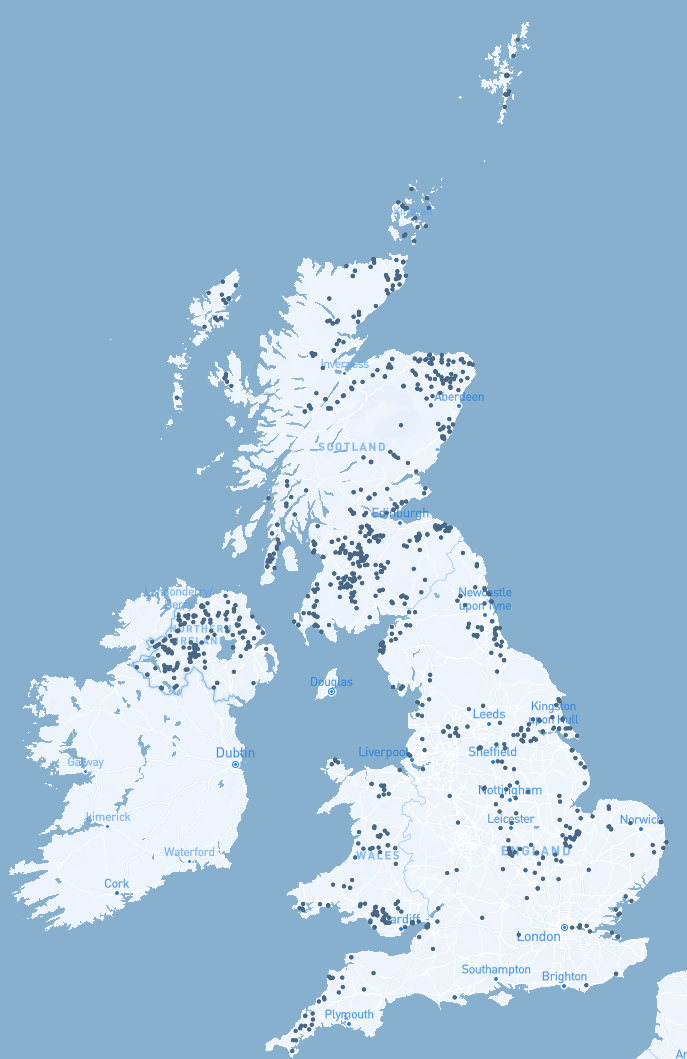
\includegraphics[height=200px]{PotentialSites.png}
    \caption{Operational or Approved Wind Farms UK 1990 - 2021,\cite{renew_database}}
    \label{fig:wind_farms}
\end{figure}

\subsection{Generation Prediction}
As we found that generation rates for wind power vary depending on a variety of weather conditions we decided that the first idea to consider to predict a new generation amount would be to use regression. This will allow us to train a model against weather data for each day with a target being  the generation a wind farm actually produced on that day. By training this on a large number of different wind farms over a large set of days, we hope to be able to accurately estimate the power generated by a wind farm for any weather pattern. We will then use this to predict a generation on an "average" day for every location to predict the performance of the proposed wind farm.\\
\noindent Currently the plan is to evaluate a few different regression models to see which finds the best fit, and in the next few weeks we will begin work on constructing the data set and conducting any feature engineering required to extract latent features from the data provided. This may not be necessary and a simple regression model against weather data may be sufficient but by testing a variety of approaches we aim to find the best result possible.
%------------------------------------------------

\section{Technical Progress}
With the majority of the time up to this point focusing on the research aspects of the project there have not been many technical developments. The main one technical aspect though is the collection of data and a start to the building of our training and testing data sets. 

\subsection{Data Collection}
From the research stage we now have a better idea of what data we are going to require to achieve the aim we set out at the beginning. There are two main things we now know to consider, a comprehensive weather breakdown for a given location at any point in time over the span of our training time range and an actual generation amount for every onshore wind farm on every day of that same training time range.
\subsubsection{Historic Weather}
In the process of searching for a good source of this weather data we came across a few potential sources. The first was the Met Office historic station data sets\cite{metoffice}. This gave us access to a selection of 37 stations across the UK, each having the the following information for every month since it's opening: \cite{metoffice}
\begin{itemize}
    \item Mean daily maximum temperature
    \item Mean daily minimum temperature
    \item Days of air frost
    \item Total rainfall 
    \item Total sunshine duration
\end{itemize}
Unfortunately this did not give us the resolution we needed nor any information on wind speeds that would seem inherently important to a discussion on wind farm performance.
\\
\noindent The option we discovered next was visualcrossing.com \cite{visualCrossing}, this website provided access to data for any location in the UK based on the closest weather stations it has access to. It gives the resolution and span of dates we need to create a comprehensive training data set. We are able to query any date and time range, at an hourly resolution getting information about:\cite{visualCrossing}
\begin{itemize}
    \item Air pressure
    \item Cloud cover
    \item Humidity
    \item Precipitation
    \item Temperature
    \item Wind speed
    \item Wind direction
    \item Wind gust speed
\end{itemize}
This amount of information should make for a plentiful feature set, hopefully allowing for a accurate prediction model to be found. The weather API system allows us to automate the data collection process although their free model limits to 1000 records a day so we are planing carefully what dates and areas we require for our data set before making any large requests.
\subsubsection{Historic Generation Amounts}
Finding values of actual generation produced by wind farms was a bit more of an involved process, from our research we have been unable to find any one specific source that gives us the full information we need. However after a bit of searching the National Grid online data portal \cite{datopian} and the Elexon Balancing Mechanism Reporting Service (BMRS) \cite{elexon} we were able to obtain a list of all wind farm Balancing Mechanism Units Ids (BMU\_IDs) which allows us to query the BMRS dashboard to obtain an actual generation amount at half hour intervals for any date it was operational. \\
\noindent This allowed us to compile a list of all the BMU\_IDs and in the next few weeks let us start to match a location, a date-time and a power output, which can be used in combination with the weather data gathered to build our data set.

%------------------------------------------------

\section{Updated Plans \& Project Management Decisions}
\subsection{Narrowed Scope}
Now we have the research completed we have a better idea of exactly what is possible for this project. Over the course of this document we have discussed some of the areas we have narrowed the scope to improve the quality of the product we do produce. For example by restricting our predictor to work initially on strictly onshore wind power we hope to ensure that our prediction accuracy can be better than if we were split across different generator types having to consider a variety of different features. \\
\noindent We believe this decision is for the best of the project as the concepts demonstrated by this more limited project will allow for expansion in the future to more easily implement other sources and locations. 
\subsection{Next Steps}
From here our project will consist of 2 main targets, the predictor system and the efficient allocation algorithm. Originally our specification planned the order such that we would implement and research the allocation algorithm before tackling the performance predictor but through the research section it became clear that this would be extremely counter intuitive. Both these components are key areas requiring a lot of focus, and they should be tackled when required instead of preemptively designing the allocation system with no performance heuristic to use with it. As such, the immediate focus now is on designing tests for the first iteration of development focused on the predictive model and then compiling the data highlighted in section 3.1 into one large training data set.\\
\subsection{Managing the project}
To keep track of each iterations development we will make use of a Kanban style board designating a iteration backlog of tasks to be done. This will help us evaluate the progress being made through the project and aim to keep a constant rate of work to ensure the project can be completed within the time frame given. In keeping with the original plan laid out in the specification most of the development work will be conducted throughout term 2 due to a reduced workload outside of the project allowing for a larger time dedication to development work.
%------------------------------------------------
\bibliographystyle{ieeetr}
\bibliography{newrefs}

\appendix

\includepdf[pages=-]{Specification(1).pdf}


\end{document}
